\section{解析}
\subsection{フィッティングの範囲指定}
今回の測定で得られたデータを$\mu$粒子が崩壊してできた電子のシンチレータへの到達時間[ns]を‎横軸に、各到達時間のイベント数を縦軸に示してフィッティングをするが、$\mu^-$は$\mu^+$より非常に短い寿命を持つ(1.1参照)ことから1000ns以下では$\mu^-$に対応する減衰曲線が無視できないと判断して1000ns以降からのデータを用いてフィッティングすることにした。

\subsection{寿命の解析}
実験aで得られたデータを1000nsから20000nsの範囲をビン数300でヒストグラムにし、それに対して関数
\begin{equation}
F(t)=A\exp\left(-\frac{t}{\tau}\right)+B
\end{equation}
でフィッティングを行う。ただし、$A,B$は定数、$\tau$は寿命である。

その結果を図\ref{mu_lifetime}に示す。
\begin{figure}[htbp]
  \centering
  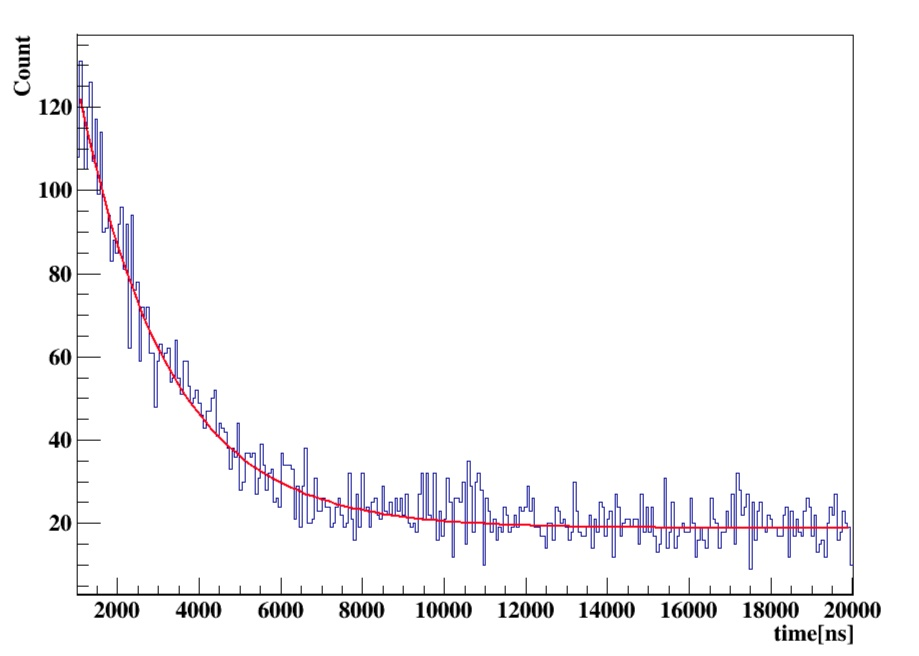
\includegraphics[width=10cm,bb=0 0 919 656]{lifetime.jpg}
  \caption{$\mu$の寿命曲線}
  \label{mu_lifetime}
\end{figure}

この結果、
\begin{align*}
A &= 170 \pm 7  \\
B &= 18.8 \pm 0.4 \\
\tau &= 2.19 \pm 0.08\,\mathrm{\mu s}
\end{align*}
を得た。このフィッティングにおける$\chi^2/\mathrm{ndf}$は1.00231であった。

\subsection{$g$因子の解析}
実験bで得られたデータを1000nsから20000nsの範囲をビン数100でヒストグラムにし、関数
\begin{equation}
G(t)=A\exp\left(-\frac{t}{\tau}\right)\exp\left(\frac{1}{2\omega\tau}\sin(\omega(t-t_0))\right)+C
\end{equation}
でフィッティングを行う。ただし、$A,B,C$は定数、$\tau$は寿命、$\omega$はスピンの歳差運動の振動数、$t_0$は初期位相を考慮した定数である。
%% その結果を図\ref{}に示す。

%% \begin{figure}
%%  \centering
%%  \includergraphics[width=5cm,clip]{}
%%  \caption{$g$因子測定の寿命曲線}
%%  \label{}
%% \end{figure}

この結果、
\begin{equation}
A= ,B= ,C= ,\tau= ,\omega= ,t_0=
\end{equation}
を得た。
